% So we make this "beamer" rather than document!

\documentclass[11pt]{beamer}
% For handout add ,handout after 11pt

\usetheme[sectionpage=none,numbering=none]{metropolis}           % Use metropolis theme
	% To do printouts, add ", handout"  after aspectratio.
\usepackage{booktabs}
\usepackage{graphicx}
\usepackage{color}

\title{Team Debriefs}
\author{\small Nick Eubank}
\date{\vspace*{.3in} \date}


% This is the beginning of a real document!
\begin{document}


\begin{frame}[c]
\maketitle
\end{frame}

\begin{frame}[c]{Psychological Safety}
\begin{figure}
    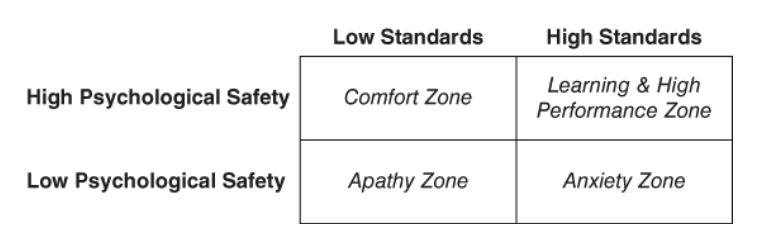
\includegraphics[width=\textwidth]{team_types.png}
\end{figure}
\pause Where do you think your team was? \\
Why do you think it ended up there? \\
What could you have done to move the team towards the top right?
\end{frame}


\begin{frame}[c]{Debrief/After Action Report}
    \begin{itemize}
        \item Constructive effort to learn and iterate
        \item Critical that lessons can be quickly put into action
        \begin{itemize}
            \item Thursday, we'll meet in our new teams and write Team Charters!
        \end{itemize}
    \end{itemize}
\end{frame}

\begin{frame}[c]{Today}
\begin{enumerate}
    \item Identify things you think went \emph{well} with your team. 
    \item Discuss \alert{why} you think they went well?
    \item Identify things you think could have gone better.
    \item Discuss \alert{how} you think you could avoid similar problems in the future?
\end{enumerate}
\end{frame}

\begin{frame}[c]{Today}
As you discuss:
\begin{itemize}
    \item Start by going around the group and letting each person speak, \alert{uninterrupted}, for around a minute. Only after everyone has had an opportunity to speak should you start processing the issues brought up.
    \item Focus on solutions (``How can we work toward making sure this goes more smoothly next time?'', ``What can we do together to make a game plan for next time?'')
    \item Be honest and if you have concerns, speak up. At the same time, however, remember to speak to \emph{your} experiences and remember to be \alert{generous and cautious} in how you interpret the actions of others.
        \begin{itemize}
            \item Remember the Fundamental Attribution Error and Naive Realism. 
            \item Remember also we're all trying to help one another.
        \end{itemize}
\end{itemize}
\end{frame}
\end{document}
